\documentclass[t,ngerman,professionalfont]{beamer}
\listfiles
\IfFileExists{beamerthemesl-it.sty}{%
  \usetheme{sl-it}
  \useoutertheme{sl-split}
}{%
  \usetheme{Luebeck}
  \usepackage{babel}
}
\usepackage[backend=biber%
  ,language=german]{biblatex}
\addbibresource{biblio.bib}
\usepackage{csquotes}
\usepackage{hologo}
\usepackage{tikz}
\usepackage{graphicx}
\graphicspath{{./img/}}
\usepackage{ifluatex}
\ifluatex%
\else%
  \usepackage[utf8]{inputenc}%
\fi

\author{Stephan Lukasczyk}
\title{\LaTeX{} im Uni-Alltag}
\subtitle{Ein \enquote{kleiner} Überblick}
\date{15.~Januar 2014}
\institute{
\includegraphics[width=3cm]{ieee-logo}\\%
  IEEE Student Branch Passau}
\begin{document}

{\usebackgroundtemplate{%
    \tikz\node[opacity=0.3]{%
      
\includegraphics[height=\paperheight,width=\paperwidth]{lion}%
    };%
  }
  \begin{frame}
    \titlepage
  \end{frame}
}

\begin{frame}
  \frametitle{Agenda}
  \tableofcontents
\end{frame}

\section{Einführung}

\begin{frame}
  \frametitle{The Name of the Game}
  \framesubtitle{Just drop a view names}
  \begin{itemize}
  \item \TeX
    \begin{itemize}
    \item Donald E. Knuth, 1978
    \item Aktuell \TeX{} 3.1415926 (März~2008)
    \item Textsatzsystem mit eingebauter\\
      Makrosprache
    \item \enquote{The \TeX{}book}
    \end{itemize}
  \item \LaTeX
    \begin{itemize}
    \item Leslie Lamport, Anfang 1980er
    \item Aktuell \hologo{LaTeX2e}
    \item Makropaket für \TeX
    \item Meistverwendetste \TeX-Variante
    \item Unzählige Literatur
    \end{itemize}
  \item CTAN (Comprehensive \TeX{} Archive Network)
    \begin{itemize}
    \item über 4\,600 Pakete
    \item \texttt{CTAN://<pkg>} für \href{http://ctan.org}{http://ctan.org/<pkg>}
    \end{itemize}
  \end{itemize}
  \begin{textblock}{3}(0.72,0.17)
    \href{https://en.wikipedia.org/wiki/File:KnuthAtOpenContentAlliance.jpg}{%
      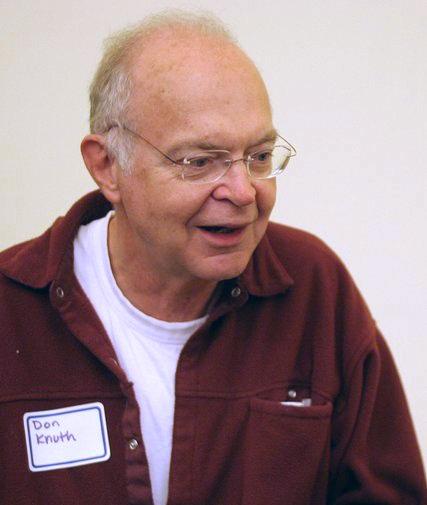
\includegraphics[width=3cm]{don-knuth}~%
      \rotatebox{90}{\tiny by Jacob Applebaum (CC-BY-SA 2.5)}%
    }
  \end{textblock}
  \begin{textblock}{3}(0.72,0.54)
    \href{https://en.wikipedia.org/wiki/File:Leslie_Lamport.jpg}{%
      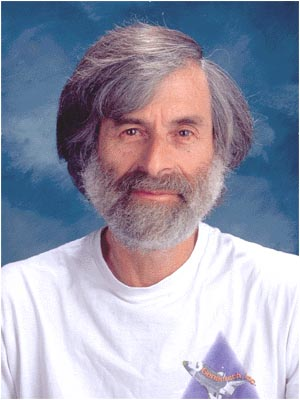
\includegraphics[width=3cm]{leslie-lamport}~%
      \rotatebox{90}{\tiny by Leslie Lamport}%
    }
  \end{textblock}
\end{frame}

\begin{frame}
  \frametitle{The Name of the Game (2)}
  \framesubtitle{Engines}
  \begin{itemize}
  \item \TeX\\
    7\,bit-ASCII, dvi-Ausgabe, v3.1415926
  \item pdf\TeX\\
    8\,bit-ASCII, dvi- oder pdf-Ausgabe, v1.40.14
  \item \hologo{XeTeX}\\
    UTF-8, Systemfonts (TTF, OTF), nur pdf-Ausgabe, schleppende
    Entwicklung, v0.9999.3
  \item \hologo{LuaTeX}\\
    UTF-8, Systemfonts (TTF, OTF), dvi- oder pdf-Ausgabe, Lua
    eingebettet, Arabischer Textsatz, v0.76
  \end{itemize}
\end{frame}

\begin{frame}
  \frametitle{Einführungen}
  \nocite{voss2012,l2short}
  \begingroup
  \printbibliography[heading=none]
  \endgroup
\end{frame}

% Fehlermeldungen
% Graphiken
% Präsentationen

{\usebackgroundtemplate{%
  \tikz\node[opacity=0.3]{%
    
\includegraphics[width=\paperwidth,height=\paperheight]{tex-background}%
  };%
}
\begin{frame}
  \frametitle{The End\dots}
  \begin{textblock}{10}(0.3,0.4)
    {\Huge\color{red}Happy \TeX-ing!}
  \end{textblock}
  \begin{textblock}{10}(0.1,0.88)
    \small All files available at
    \href{https://github.com/sl-gap/tex-tutorial/}{https://github.com/sl-gap/tex-tutorial/}
  \end{textblock}
\end{frame}
}

\end{document}

%%% Local Variables: 
%%% mode: latex
%%% coding: utf-8
%%% TeX-engine: luatex
%%% TeX-PDF-mode: t
%%% TeX-master: t
%%% End: 
